\subsection{Dynamic Programming Formulation}
The dynamic programming can be done in two different ways: top down and bottom up. We will try to implement the formulation when we go from bottom to up. It means we will iteratively add values to the profitable revenue from bottom and take the length i which will maximize our one step ahead revenue. We will continue doing this until we finish the length.
	

\subsection{Implementation}
	The code will be given below. For $n=96$ and $n=100$, we got 210 and 220 respectively.

\subsection{Asymptotic Computational Complexity}
	The big O computational complexity of our dynamic programming function will be $O(n)$ as we will have two loops one goes 1 to n, second is a constant number. 

\subsection{Runtime Analysis}

	The figure below represents the runtime for \code{n = 1:1:100}. It is the result as we predicted. Time should should grow linearly as n increases. 
	
		\begin{figure}[H]
		\centering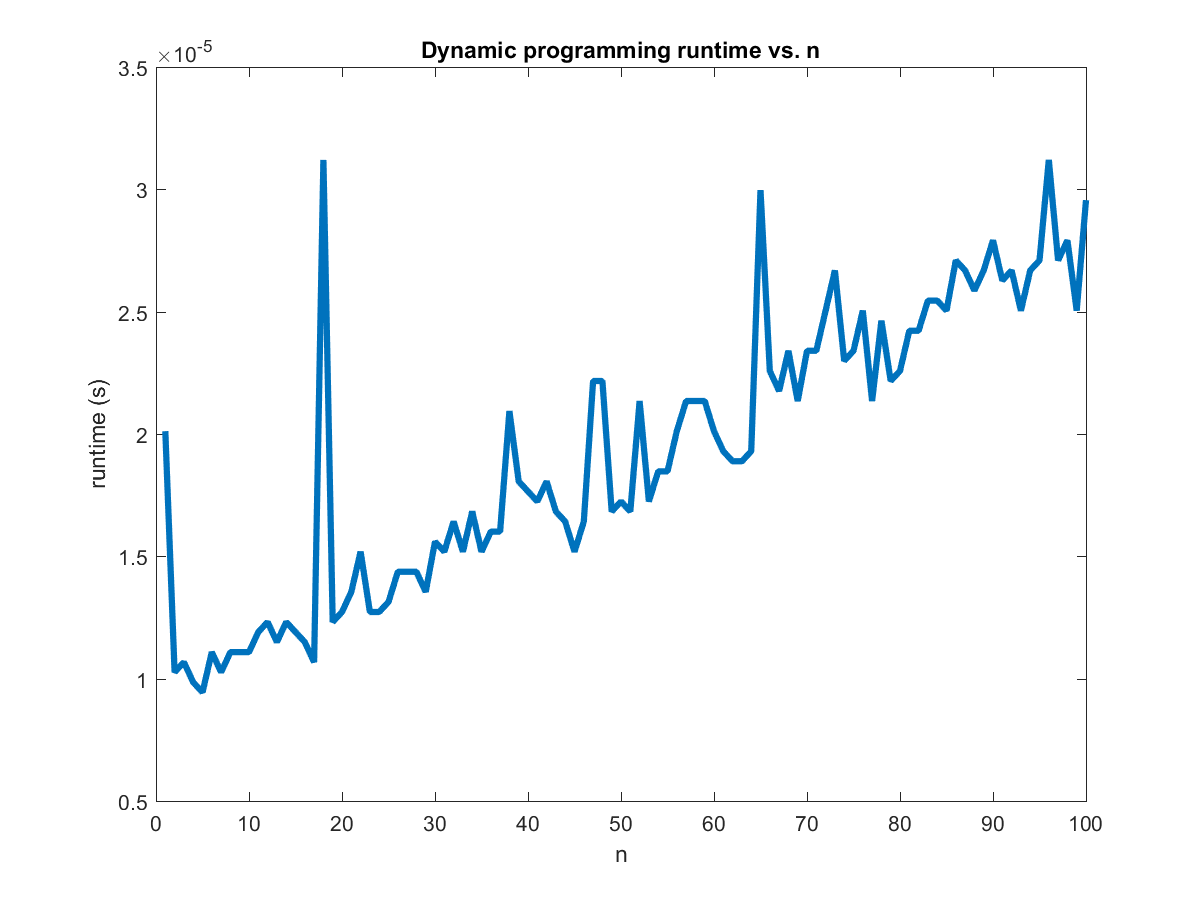
\includegraphics[width=0.6\textwidth]{pr2_timing}
		\caption{Dynamic programming runtime vs. n.}
		\end{figure}